\RequirePackage{ifluatex}
\ifluatex
\documentclass[lualatex,aspectratio=54,12pt,]{beamer}
\else
\documentclass[aspectratio=169,15pt,]{beamer}
\fi
%%% aspectratio
% 1610
% 169
% 149
% 141  (1,41:1)
% 54
% 43 (default)
% 32

\usepackage{lipsum}

\input{\jobname .ltx}

\usefonttheme{professionalfonts} 

% \usepackage{pgfpages}
% \pgfpagesuselayout{4 on 1}[a4paper,landscape,border shrink=10mm]
% \usepackage{lmodern}
\usepackage{xcolor}
\usepackage{bookmark}

\ifluatex
\usepackage[]{fontspec}
\setsansfont{Carlito}[Numbers=OldStyle]  % lub Numbers=Lining
\else
\usepackage[utf8]{inputenc}
\usepackage[T1]{fontenc}
\usepackage{carlito}
\fi

\renewcommand{\partname}{Część} % Zmiana "Part" na "Część"

\title{Zastosowanie dużych modeli językowych do wykrywania i naprawiania błędów bezpieczeństwa i podatności w kodzie aplikacji webowych}
\subtitle{Application of Large Language Models to Detection and Correction Security Breaches and Threats in Web Application Source Codes}
\author[Patryk Fidler]{Patryk Fidler \\ \texttt{259468@student.pwr.edu.pl}}
%\coauthor[dr hab. inż. Maciej Piasecki]{Promotor: dr hab. inż. Maciej Piasecki \\Jednostka prowadząca: [Katedra Sztucznej Inteligencji][Wydział Informatyki i Telekomunikacji]}
\institute{Promotor: dr hab. inż. Maciej Piasecki \\Jednostka prowadząca: Katedra Sztucznej Inteligencji, Wydział Informatyki i Telekomunikacji \\Department of Artificial Intelligence, Faculty of Computer Science and Telecommunications}
%\date[ISPN ’80]{Seminarium dyplomowe 2}
\date{\today}
% \pgfdeclareimage[height=\paperheight,width=\paperwidth]{TG}{flower} 
% \titlegraphic{\pgfuseimage{TG}}
\usetheme[vertical,lang=en,hr=true,pagenumbers,navigation]{NewPwr}
% \usetheme{Warsaw}
%\setbeamercolor*{block title}{fg=Logo,bg=Logo!20}
%\setbeamercolor*{block body}{fg=black,bg=Logo!10}

\begin{document}

\begin{frame}
 \titlepage
\end{frame}

\frame{\tableofcontents}

\section{Cel pracy}

\begin{frame}{Cel pracy}
      \begin{itemize}
        \item Opracowanie praktycznych rozwiązań do statycznej analizy kodu dla aplikacji webowych.
        \item Badanie skuteczności dużych modeli językowych w wykrywaniu podatności i luk bezpieczeństwa.
      \end{itemize}
\end{frame}


\section{Zakres pracy}

\begin{frame}{Zakres pracy}
      \begin{enumerate}
        \item Analiza istniejącej literatury i badań, w szczególności artykułu "Can OpenAI Codex and Other Large Language Models Help Us Fix Security Bugs?".
        \item Projektowanie i implementacja narzędzia do statycznej analizy kodu opartego na modelach OpenAI.
        \item Przygotowanie zbioru danych z kodem zawierającym potencjalne podatności.
        \item Testowanie i porównanie skuteczności z innymi rozwiązaniami, np. oferowanymi przez firmę Snyk.
        \item Analiza wyników i formułowanie wniosków.
      \end{enumerate}
\end{frame}

\section{Wyniki realizacji pracy}
\section{Podsumowanie}
\section{Literatura}
\part{Wyniki realizacji pracy}
\section{Wyniki realizacji pracy}

\begin{frame}
      \partpage
\end{frame}

\begin{frame}
      \frametitle{Wyniki realizacji pracy}
      \framesubtitle{Założenia, dane wejściowe, kryteria oceny}
      \begin{itemize}
        \item Założenie: Wykorzystanie modeli GPT-3.5, GPT-4, Llama2-code do analizy bezpieczeństwa kodu.
        \item Dane wejściowe: Kody źródłowe aplikacji z potencjalnymi błędami bezpieczeństwa.
        \item Kryteria oceny: Skuteczność wykrywania podatności takich jak: \\ \scriptsize Authentication Bypass, Code Injection, Format String Attacks, Integer Overflow, NoSQL Injection, Path Traversal, Prototype Pollution, Resource Injection, 
        SQL Injection, Unsafe Deserialization, XSS Buffer Overflow, Command Injection, Denial Of Service, IDOR LDAP Injection, Open Redirect, PHP Object Injection, Sensitive Data Exposure, SSRFUse After Free, XXE Code Execution, Connection String Injection, 
        File Inclusion, Insecure File Uploads, Log Forging Out of Bounds, PostMessage Security, ReDoS Server Side Template Injection, Symlink Attack, XPATH Injection, Zip Traversal oraz inne.
      \end{itemize}
\end{frame}

\begin{frame}
      \frametitle{Wyniki realizacji pracy}
      \framesubtitle{Metody i rozwiązania}
      \begin{itemize}
        \item Efektem końcowym jest autonomiczny
        system umożliwiający statyczną analizę kodu
        źródłowego oraz wynik badawczy składający
        się z macierzy błędów, porównania
        efektywności poszczególnych modeli oraz
        wykresy skuteczności w różnych
        technologiach programistycznych. 
      \end{itemize}
\begin{columns}
      \scriptsize
        \begin{column}{0.5\textwidth}
          \textbf{Metody:}
          \begin{itemize}
            \item Algorytmy fragmentowania
            \item In-context learning (uczenie się w kontekście)
            \item Retrieval Augmented Generation - RAG (napisany własny kod, w tej chwili dostępne jest za pomocą OpenAI Assistant API)
            \item Analiza porównawcza
          \end{itemize}
        \end{column}
      \begin{column}{0.5\textwidth}
      \textbf{Środki:}
      \begin{itemize}
        \item Modele językowe GPT-3.5, GPT-4
        \item Ollama - środowisko kontenerowe dla modeli językowych, łatwe w użyciu otwartoźródłowe modele językowe
        \item OpenAI Assistant API 
        \item Zbiór danych z kodem zawierającym podatności
        \item statyczne testy podatności jak CodeQL
        \item Istniejące rozwiązania komercyjne - Snyk
        \item Python 3.12
        \item Komputer osobisty
      \end{itemize}
      \end{column}
  \end{columns}
\end{frame}

\begin{frame}
      \frametitle{Wyniki realizacji pracy}
      \framesubtitle{Schematy i wyniki}
      \begin{figure}
            \centering
            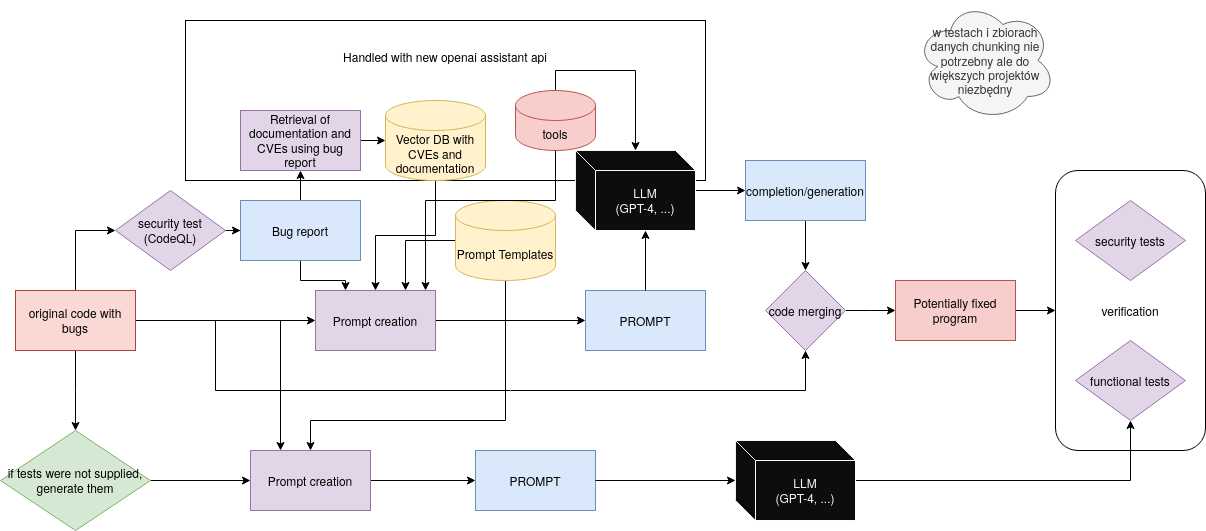
\includegraphics[width=0.9\linewidth]{gptester.drawio.png}
            \caption{Schemat blokowy działania programu GPTester}
      \end{figure}

\end{frame}

\begin{frame}
      \frametitle{Wyniki realizacji pracy}
      \framesubtitle{Oprogramowanie}
      \begin{figure}
            \centering
            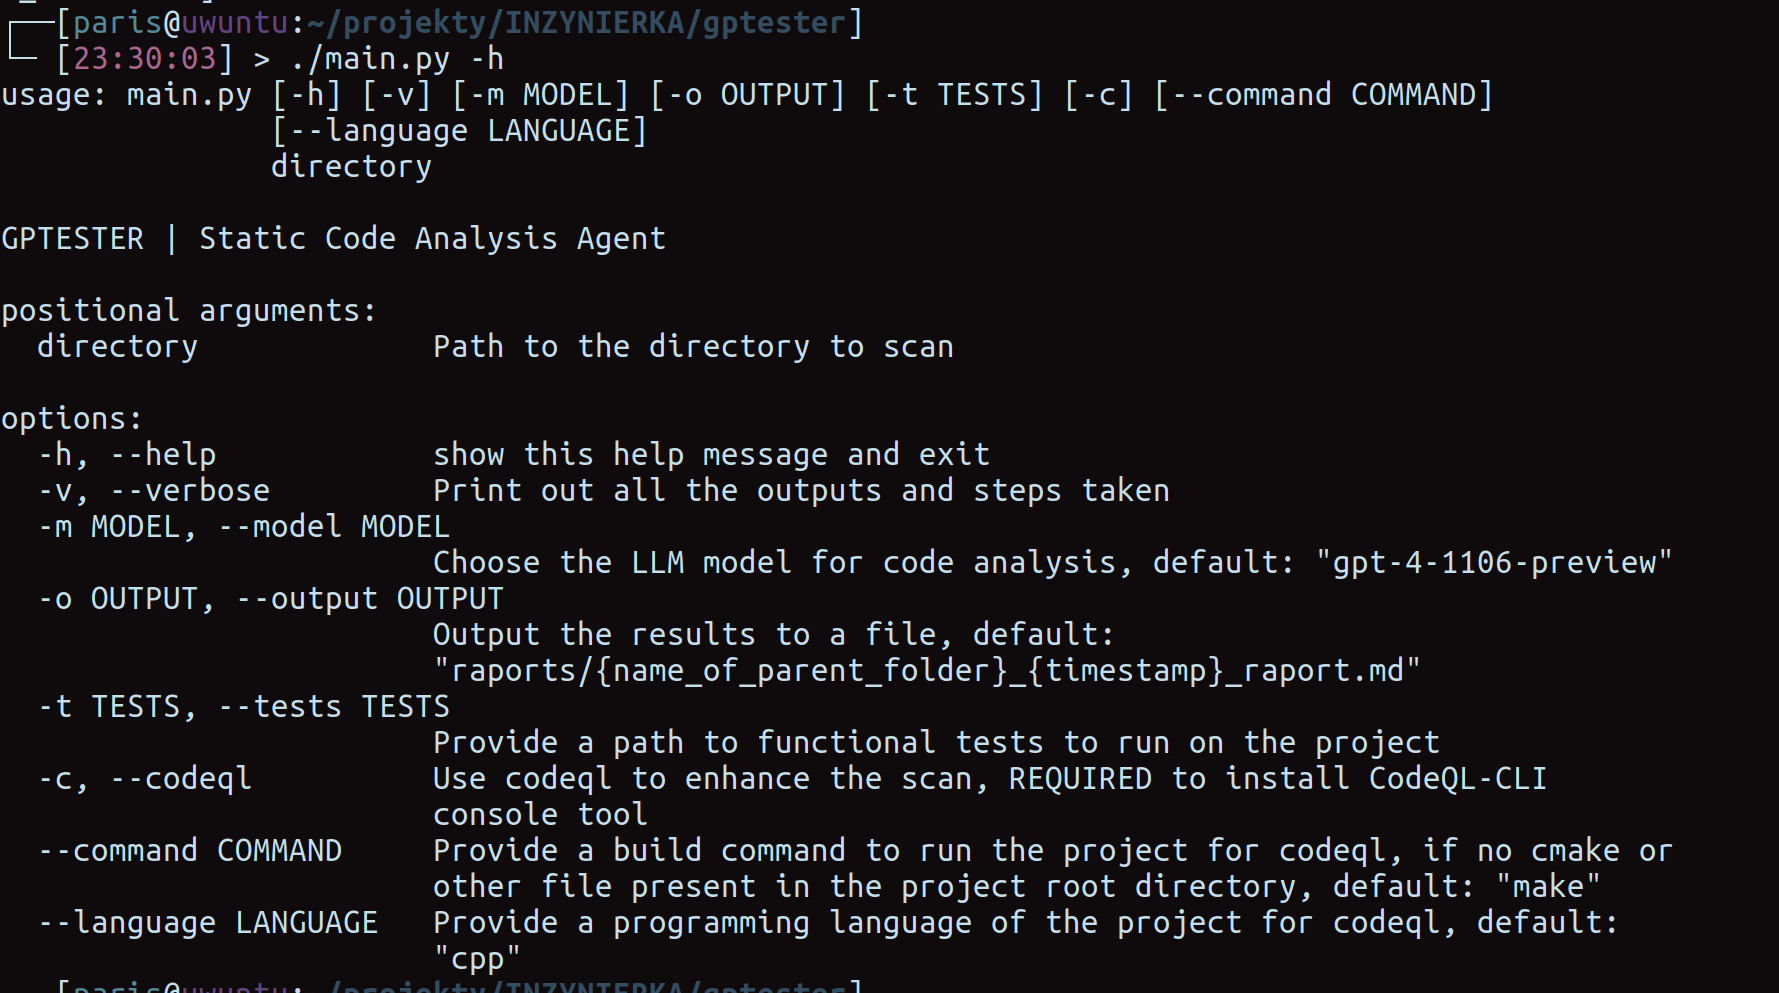
\includegraphics[width=0.6
            \linewidth]{gptester-h.png}
            \caption{Użycie programu GPTester}
      \end{figure}

      \begin{block}{repozytorium projektu}
            https://github.com/70ziko/gptester
      \end{block}
\end{frame}

\begin{frame}
      \frametitle{Wyniki realizacji pracy}
      \framesubtitle{Oprogramowanie}
      \begin{figure}
            \centering
            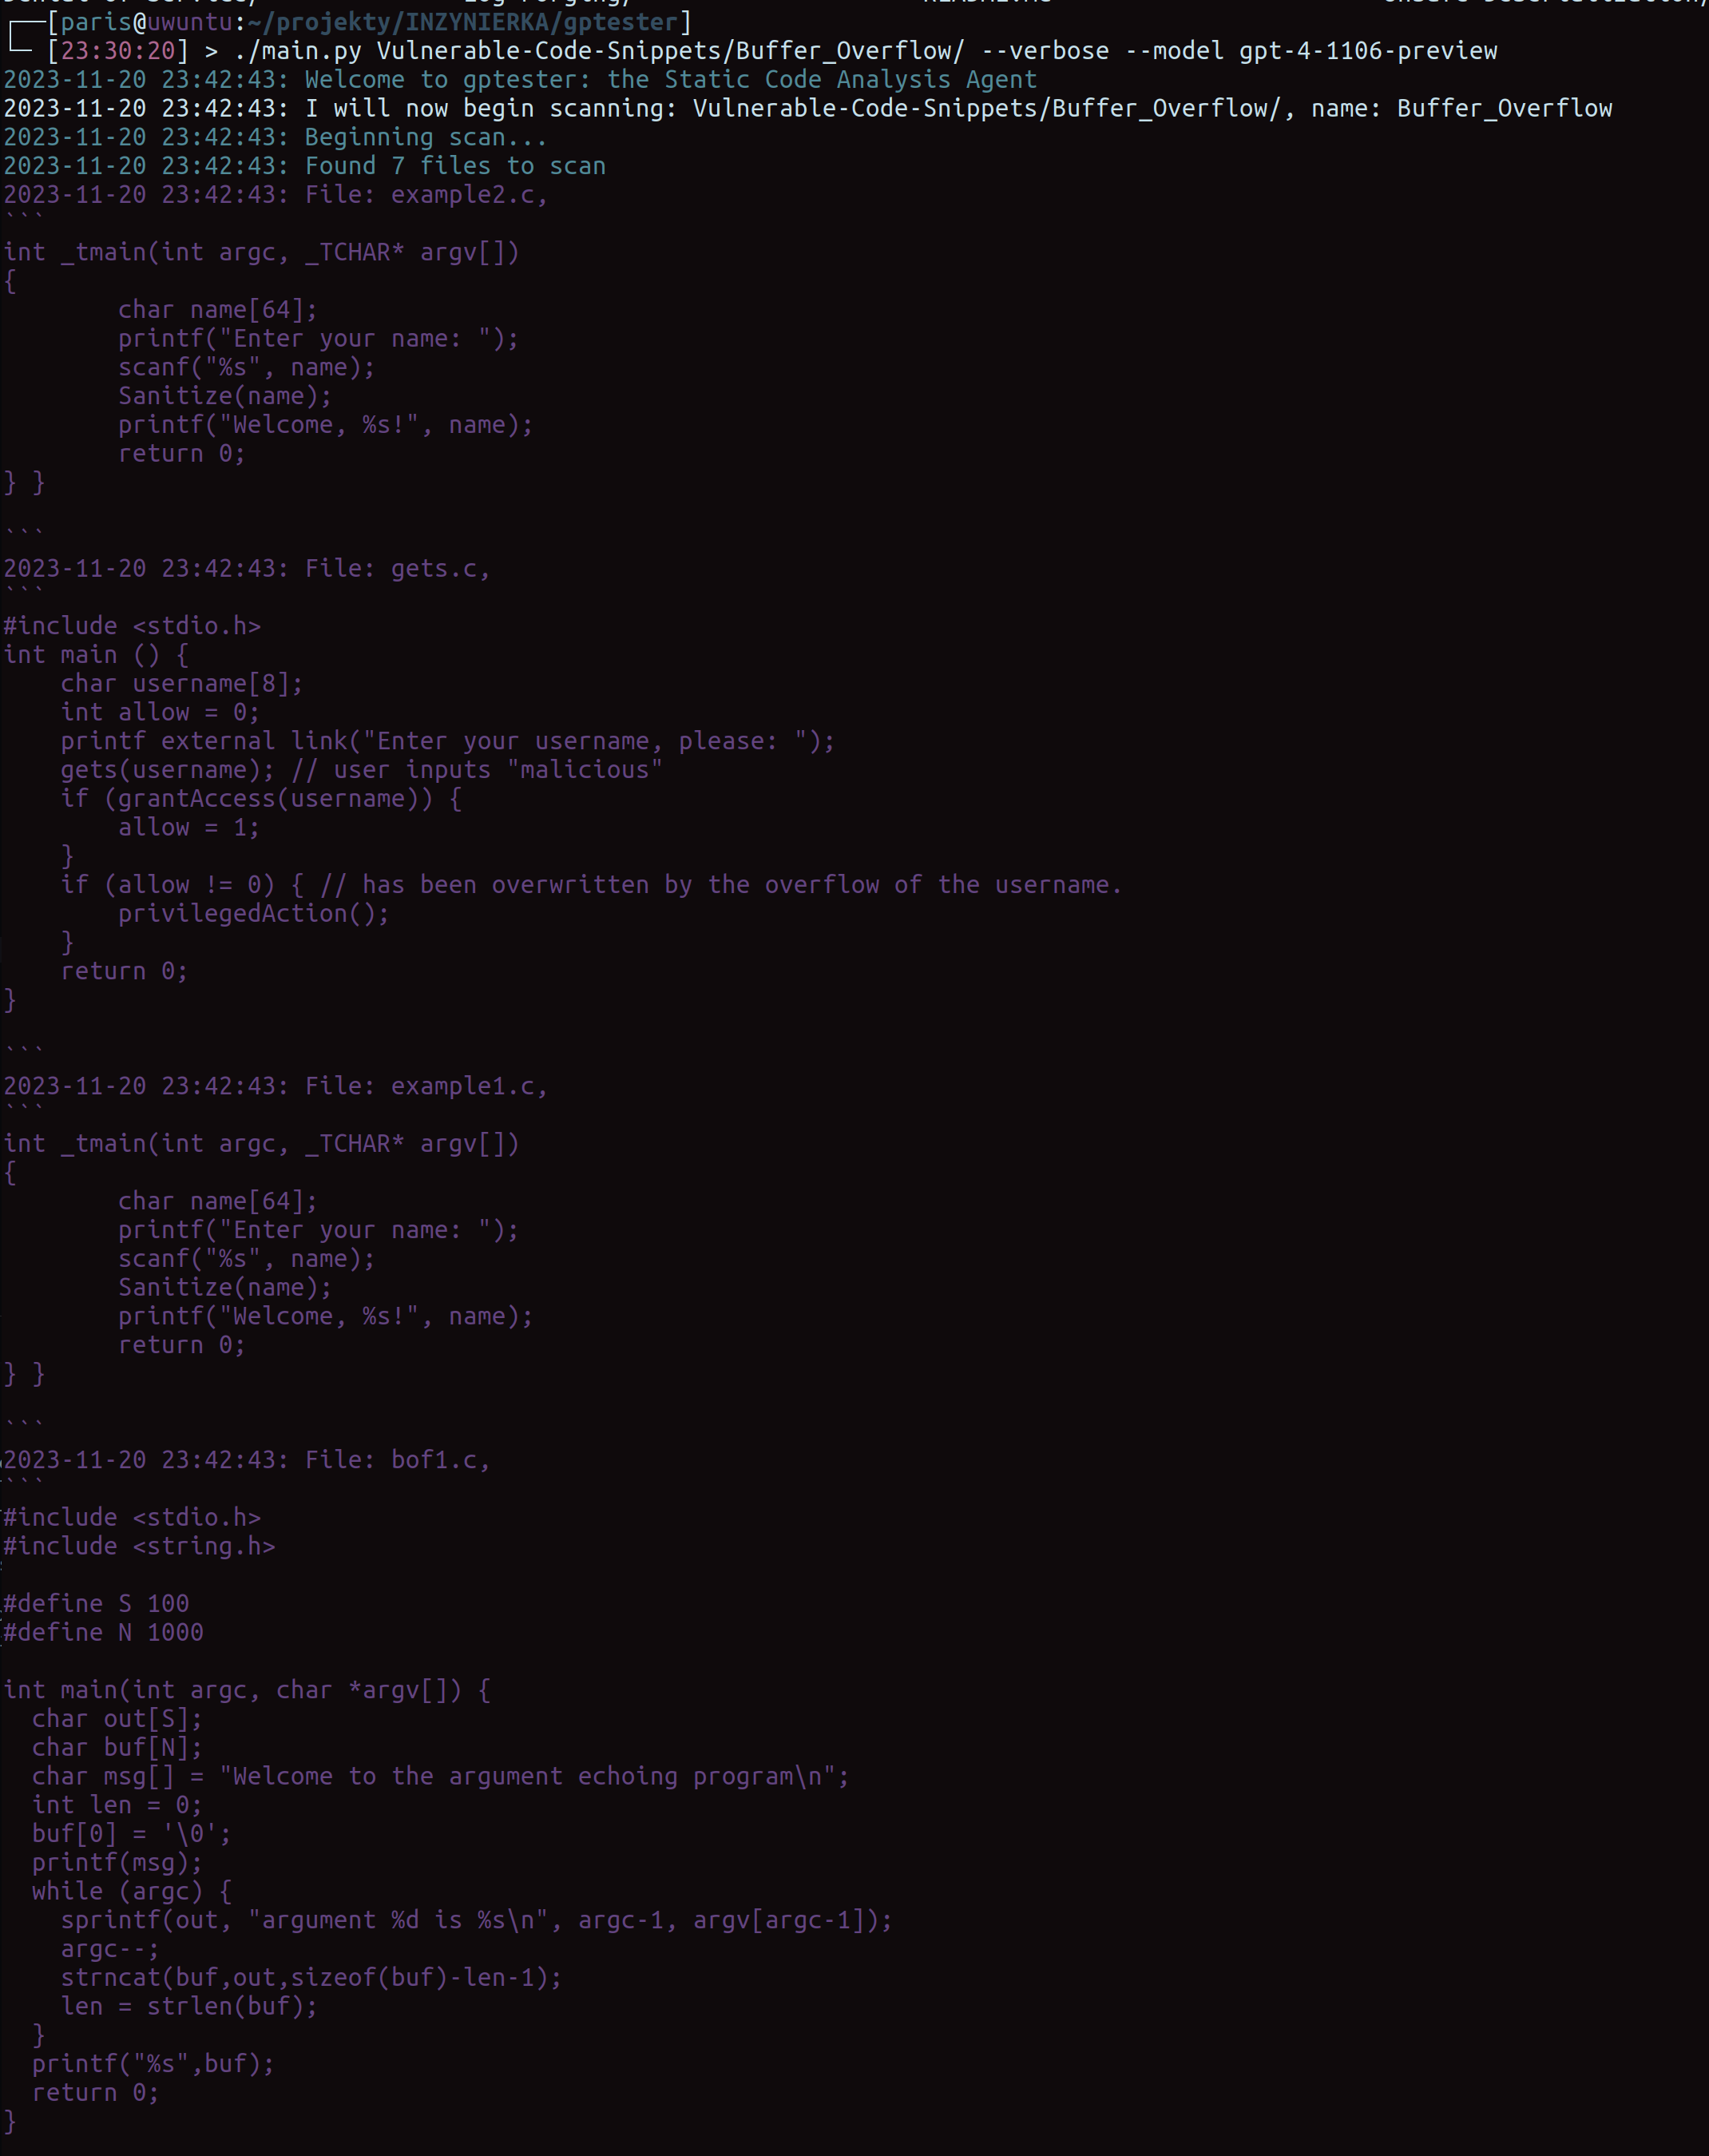
\includegraphics[width=0.6
            \linewidth]{gptester1.png}
            \caption{Użycie programu GPTester}
      \end{figure}

\end{frame}

\begin{frame}
      \frametitle{Wyniki realizacji pracy}
      \framesubtitle{Oprogramowanie}
      \begin{figure}
            \centering
            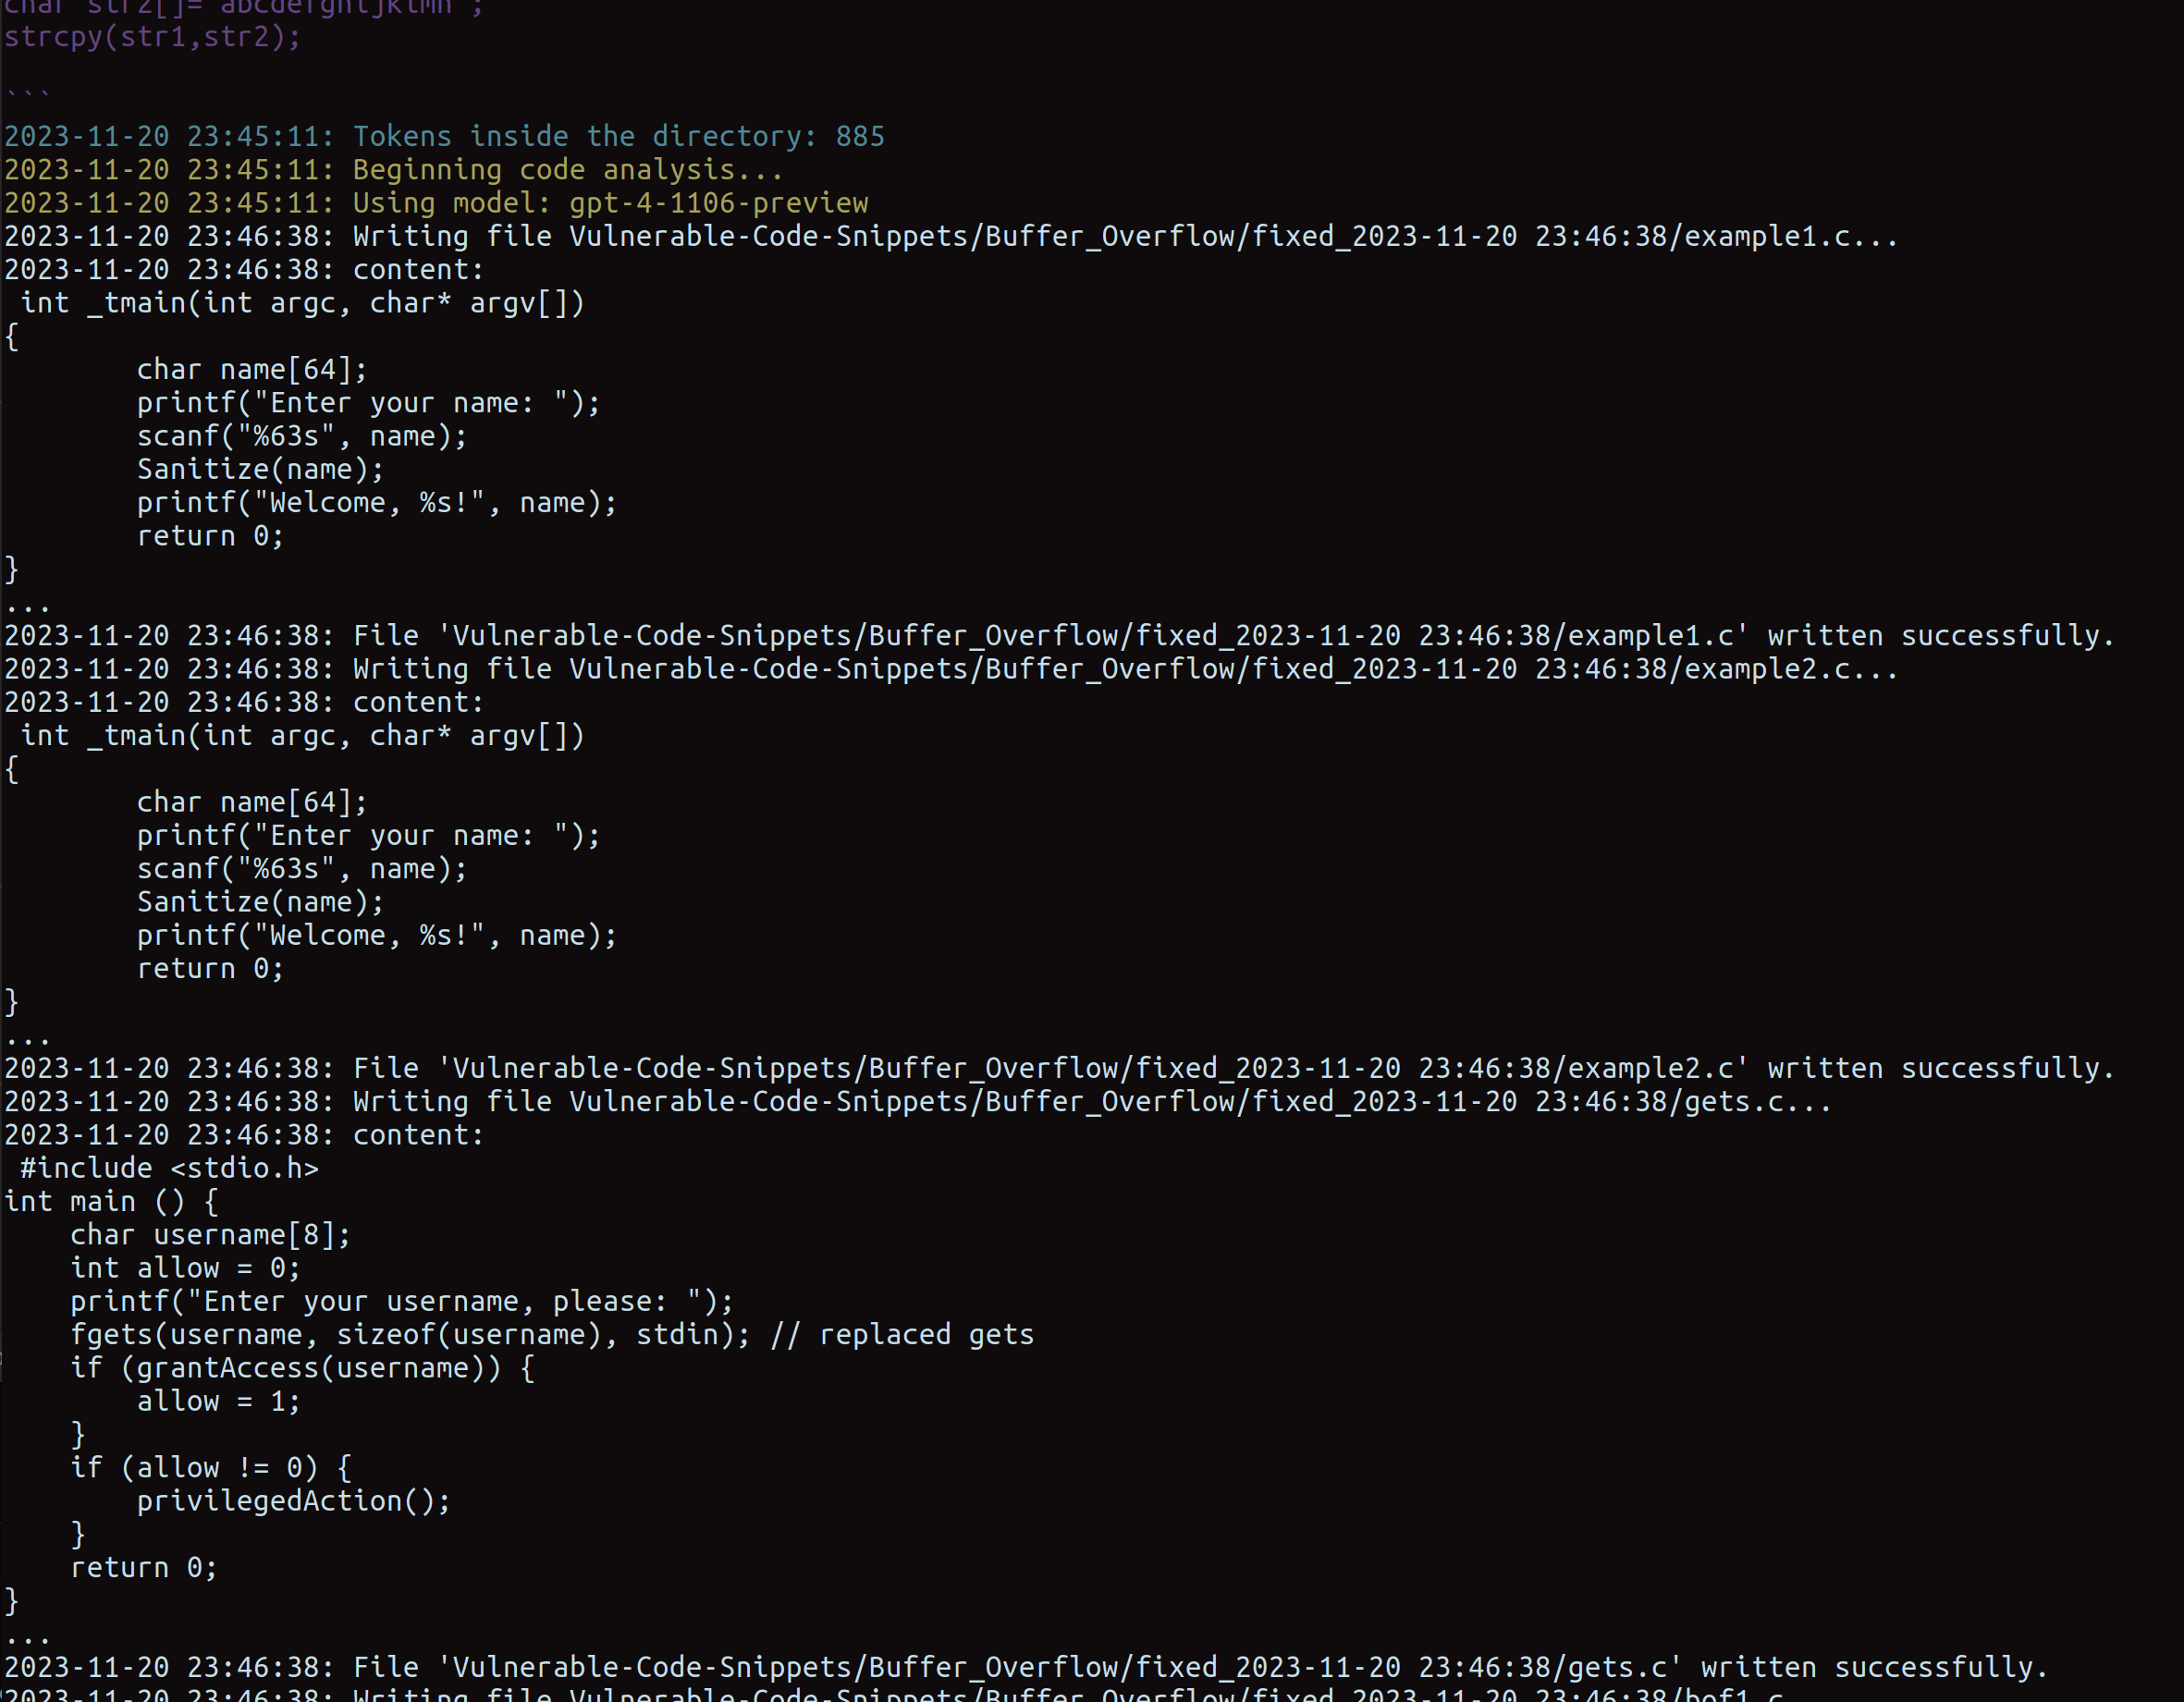
\includegraphics[width=0.6
            \linewidth]{gptester2.png}
            \caption{Użycie programu GPTester}
      \end{figure}

\end{frame}

\begin{frame}
      \frametitle{Wyniki realizacji pracy}
      \framesubtitle{Oprogramowanie}
      \begin{figure}
            \centering
            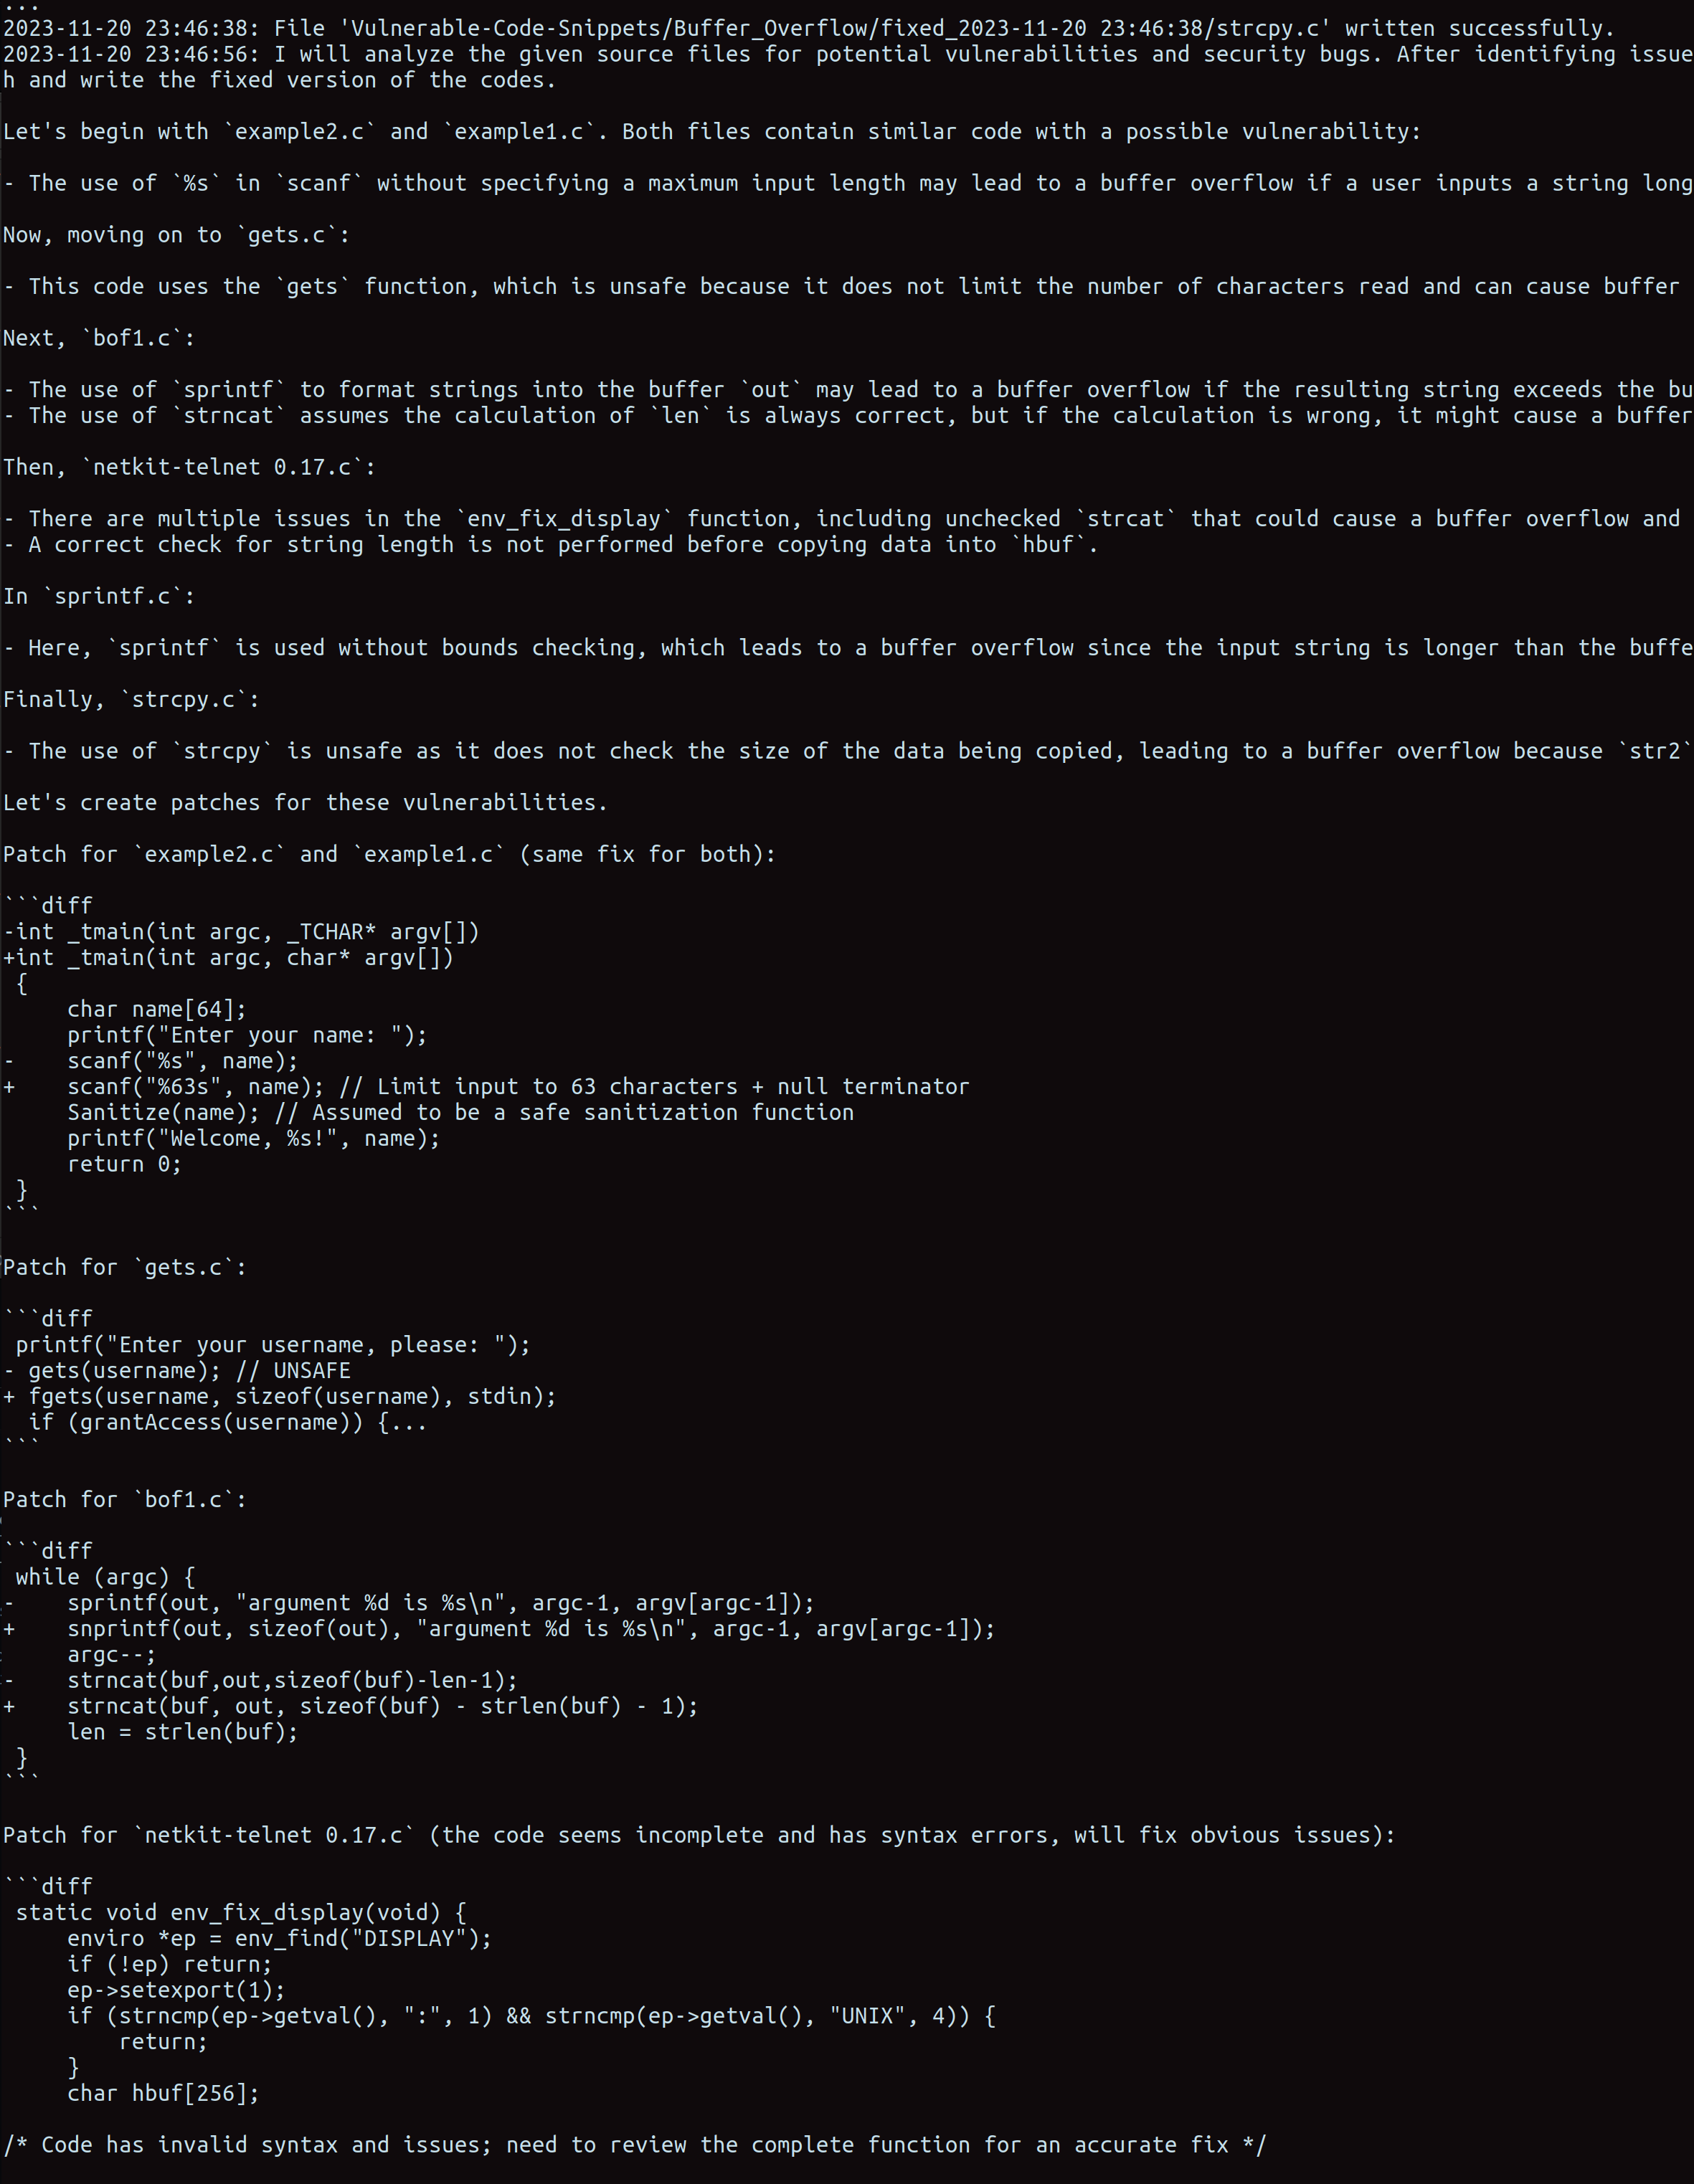
\includegraphics[width=0.4
            \linewidth]{gptester3.png}
            \caption{Użycie programu GPTester}
      \end{figure}

\end{frame}

\begin{frame}[fragile]
      \frametitle{Wyniki realizacji pracy}
      \framesubtitle{Oprogramowanie - Podsumowanie napraw}
      \scriptsize
      \begin{verbatim}
        2023-11-20 23:46:56: All the files with identified vulnerabilities have 
        been fixed and written to the "fixed" folder successfully. Here is a summary 
        of the changes made:
    
        - `example1.c` and `example2.c`: Usage of `%s` in `scanf` replaced with `%63s` 
          to prevent buffer overflow.
        - `gets.c`: Replaced `gets` with `fgets` to prevent buffer overflow.
        - `bof1.c`: Replaced `sprintf` with `snprintf` and corrected the buffer 
          length check in `strncat` to prevent buffer overflow.
        - `sprintf.c`: Increased buffer size by 1 to account for the null terminator 
          and replaced `sprintf` with `snprintf` to prevent buffer overflow.
        - `strcpy.c`: Replaced `strcpy` with `strncpy` and ensured null termination 
          to prevent buffer overflow.
        - `netkit-telnet 0.17.c`: Indicated that the code is incomplete and has 
          syntax errors; thus, a complete function context is required for an 
          accurate fix. The current changes are placeholders and do not form a 
          functional fix.
    
        The `netkit-telnet 0.17.c' file needs a complete review of the function 
        `env_fix_display` for an accurate fix, as the code snippet has syntax errors 
        and seems to be cut off.
    
        Please note that the file `netkit-telnet 0.17.c' within the fixed folder 
        contains a comment indicating the need for further review rather than a 
        functional fix.
      \end{verbatim}
    \end{frame}

    \begin{frame}[fragile]
      \frametitle{Wyniki realizacji pracy}
      \framesubtitle{Oprogramowanie - Szczegółowa analiza i łatki}
      \tiny
      \begin{verbatim}
        2023-11-20 23:46:56: I will analyze the given source files for potential 
        vulnerabilities and security bugs. After identifying issues, I will provide 
        the git format patch and write the fixed version of the codes.
    
        Let's begin with `example2.c' and `example1.c`. Both files contain similar 
        code with a possible vulnerability:
        ...
    
        Finally, `strcpy.c`:
        ...
    
        Let's create patches for these vulnerabilities.
    
        Patch for `example2.c' and `example1.c' (same fix for both):
      \end{verbatim}
    \begin{verbatim}
    -int _tmain(int argc, _TCHAR* argv[])
    +int _tmain(int argc, char* argv[])
     {
         char name[64];
         printf("Enter your name: ");
    -    scanf("%s", name);
    +    scanf("%63s", name); // Limit input to 63 characters + null terminator
         Sanitize(name); // Assumed to be a safe sanitization function
         printf("Welcome, %s!", name);
         return 0;
     }
    \end{verbatim}

    Patch for `gets.c`:

    \begin{verbatim}
     printf("Enter your username, please: ");
    - gets(username); // UNSAFE
    + fgets(username, sizeof(username), stdin);
      if (grantAccess(username)) {...
    \end{verbatim}

    Patch for `bof1.c`:

    \begin{verbatim}
     while (argc) {
    -    sprintf(out, "argument %d is %s\n", argc-1, argv[argc-1]);
    +    snprintf(out, sizeof(out), "argument %d is %s\n", argc-1, argv[argc-1]);
         argc--;
    -    strncat(buf,out,sizeof(buf)-len-1);
    +    strncat(buf, out, sizeof(buf) - strlen(buf) - 1);
         len = strlen(buf);
     }
    \end{verbatim}
    
        I will proceed to create the fixed version of these files.

\end{frame}
    
    
\begin{frame}
      \frametitle{Wyniki realizacji pracy}
      \framesubtitle{Analiza i wnioski}
      \begin{itemize}
            \item Model GPT-4 poprawnie radzi sobie ze znajdowaniem podatności w kodzie.
            \item GPT-4 w najnowszej wersji bardzo dobrze potrafi używać dostarczonych mu narzędzi i funckji.
            \item Dalsze testy są potrzebne, aby określić skuteczność modelu GPT-4 oraz innych modeli w wykrywaniu podatności w kodzie.
      \end{itemize}

\end{frame}

\section{Podsumowanie}
\part{Podsumowanie}

\begin{frame}
      \partpage
\end{frame}

\begin{frame}
      \frametitle{Podsumowanie}
      \framesubtitle{Wnioski oraz postęp w osiągnięciu celu}
      \begin{itemize}
            \item Sukces implementacji praktycznego rozwiązania statycznej analizy kodu.
            \item Potwierdzono bardzo dobre zdolności modeli do używania kontekstu, narzędzi i wiedzy z uczenia podstawowego w wykrywaniu podatności.
            \item Napisano własny kod do Generowania rozszerzonego pozyskiwaniem danych - Retrieval Augmented Generation.
            \item \alert{Przystosowanie programu dla dużych projektów.}
            \item \alert{Badanie skuteczności dużych modeli językowych w wykrywaniu podatności i luk bezpieczeństwa.}
            \item \alert{Analiza porównawcza skuteczności modeli językowych w wykrywaniu podatności w różnych stosach technologicznych.}
            \item \alert{Opracowanie wyników badań, stworzenie przejrzystych wykresów oraz wniosków.}
      \end{itemize}
      \textbf(Została osiągnięta większość założonych celów.)
\end{frame}

\section{Literatura}

\begin{frame}
      \frametitle{Literatura}
      \begin{itemize}
           \item ``Can OpenAI Codex and Other Large Language Models Help Us Fix Security Bugs?'' - Hammond Pearce, Benjamin Tan, Baleegh Ahmad, Ramesh Karri, Brendan Dolan-Gavitt. Wydawnictwo: Cornell University
           \item ``Examining Zero-Shot Vulnerability Repair with Large Language Models'' - Hammond Pearce, Benjamin Tan, Baleegh Ahmad, Ramesh Karri, Brendan Dolan-Gavitt. Wydawnictwo: 2023 IEEE Symposium on Security and Privacy
           \item ``Assisting Static Analysis with Large Language Models: A ChatGPT Experiment'' - Haonan Li, Yu Hao, Yizhuo Zhai, Zhiyun Qian. \url{https://www.cs.ucr.edu/~zhiyunq/pub/fseivr23_static_chatgpt.pdf}
           \item ``Detecting Code Vulnerabilities with Large Language Models (LLMs)'' - Ravi Lingarkar. \url{https://www.linkedin.com/pulse/detecting-code-vulnerabilities-large-language-models-llms-lingarkar}
           \item \url{https://github.com/chris-koch-penn/gpt3_security_vulnerability_scanner}
         \end{itemize}
\end{frame}


\begin{frame}
      \frametitle{Zakończenie prezentacji}
      \centering % Centruje tekst
      \Huge % Duża czcionka
      % \textcolor{Maroon}{Dziękuję za uwagę.} % Tekst w kolorze bordowym
      \textcolor{Logo}{Dziękuję za uwagę.} % Tekst w kolorze Logo
\end{frame}

\end{document}

\section{Raz}

\begin{frame}
 \frametitle{There Is No Largest Prime Number}
 \framesubtitle{The proof uses \textit{reductio ad absurdum}.}
 \begin{theorem}
  There is no largest prime number. 
  \end{theorem}
  \begin{proof}%[Dowód]
 \begin{enumerate}
  \item<1-| alert@1> Suppose $p$ were the largest prime number.
  \item<2-> Let $q$ be the product of the first $p$ numbers.
  \item<3-> Then $q+1$ is not divisible by any of them.
  \item<1-> But $q + 1$ is greater than $1$, thus divisible by some prime
        number not in the first $p$ numbers.
 \end{enumerate}
 \end{proof}
\end{frame}

\begin{frame}{A longer title}
 \begin{itemize}
  \item one
  \item two
 \end{itemize}
\end{frame}

\section{dwa}

\begin{frame}{Lista punktowana}
 \begin{itemize}
  \item
        Item 1
  \item
        Item 2
  \item
        Item 3
  \item
        \alert{Alerted item}
 \end{itemize}
\end{frame}

\subsection{trzy}

\begin{frame}
 \frametitle{Lista numerowana}
 \begin{enumerate}
  \item
        Item 1
  \item
        Item 2
  \item
        Item 3
  \item
        \alert{Alerted item}
 \end{enumerate}
\end{frame}

\subsection{cztery}

\begin{frame}
 \frametitle{Blok}
 alertblock:
 \begin{alertblock}{Tytuł}
  Zawartość
 \end{alertblock}

 exampleblock:
 \begin{exampleblock}{Tytuł}
  Przykład Przykład Przykład Przykład Przykład Przykład Przykład Przykład Przykład Przykład Przykład Przykład Przykład Przykład Przykład Przykład Przykład Przykład Przykład Przykład
 \end{exampleblock}

 zwykły blok
 \begin{block}{Tytuł}
 Przykład, przykład, przykład…
 \end{block}

 alertenv:
 \begin{alertenv}<2>
  (environment contents)
 \end{alertenv}
\end{frame}

\part{Lipsum}

\begin{frame}
      \partpage
\end{frame}

\begin{frame}[allowframebreaks=0.97]{Długi Tekst}
 \lipsum
\end{frame}

\begin{frame}[plain,c]
plain slide
\end{frame}

\begin{frame}{Ostatni slajd}
ala ma 
\end{frame}
\end{document}
